\documentclass[unicode,11pt,a4paper,oneside,numbers=endperiod,openany]{scrartcl}
\newcommand\tab[1][0.5cm]{\hspace*{#1}}
\usepackage{array}
\usepackage{multirow}
\usepackage{graphicx}
\usepackage[utf8]{inputenc}
\usepackage{listings}
\usepackage{xcolor}
\usepackage{seqsplit}
\usepackage{float}
\usepackage{booktabs}
\usepackage{subcaption}
\usepackage{adjustbox}
%New colors defined below
\definecolor{codegreen}{rgb}{0,0.6,0}
\definecolor{codegray}{rgb}{0.5,0.5,0.5}
\definecolor{codepurple}{rgb}{0.58,0,0.82}
\definecolor{backcolour}{rgb}{0.98,0.98,0.98}
%Code listing style named "mystyle"
\lstdefinestyle{mystyle}{
  backgroundcolor=\color{backcolour}, commentstyle=\color{codegreen},
  keywordstyle=\color{magenta},
  numberstyle=\tiny\color{codegray},
  stringstyle=\color{codepurple},
  basicstyle=\ttfamily\footnotesize,
  breakatwhitespace=false,         
  breaklines=true,                 
  captionpos=b,                    
  keepspaces=true,                 
  numbers=left,                    
  numbersep=5pt,                  
  showspaces=false,                
  showstringspaces=false,
  showtabs=false,                  
  tabsize=2,
  numbers=none
}
\lstdefinestyle{base}{
  language=C,
  emptylines=1,
  breaklines=true,
  basicstyle=\ttfamily\color{black},
  moredelim=**[is][\color{red}]{@}{@},
}
\lstset{style=mystyle}
\newcommand\MyBox[2]{
  \fbox{\lower0.75cm
    \vbox to 1.7cm{\vfil
      \hbox to 1.7cm{\hfil\parbox{1.4cm}{#1\\#2}\hfil}
      \vfil}%
  }%
}
\usepackage{ifthen}
\usepackage[utf8]{inputenc}
\usepackage{graphics}
\usepackage{graphicx}
\usepackage{hyperref}

\pagestyle{plain}
\voffset -5mm
\oddsidemargin  0mm
\evensidemargin -11mm
\marginparwidth 2cm
\marginparsep 0pt
\topmargin 0mm
\headheight 0pt
\headsep 0pt
\topskip 0pt        
\textheight 255mm
\textwidth 165mm

\newcommand{\duedate} {}
\newcommand{\setduedate}[1]{%
\renewcommand\duedate {Due date:~ #1}}
\newcommand\isassignment {false}
\newcommand{\setassignment}{\renewcommand\isassignment {true}}
\newcommand{\ifassignment}[1]{\ifthenelse{\boolean{\isassignment}}{#1}{}}
\newcommand{\ifnotassignment}[1]{\ifthenelse{\boolean{\isassignment}}{}{#1}}

\newcommand{\assignmentpolicy}{
\begin{table}[h]
\begin{center}
\scalebox{0.8} {%
\begin{tabular}{|p{0.02cm}p{16cm}|}
\hline
&\\
\multicolumn{2}{|c|}{\Large\textbf{HPC  2022 ---  Submission Instructions}}\\
\multicolumn{2}{|c|}{\large\textbf{(Please, notice that following instructions are mandatory: }}\\
\multicolumn{2}{|c|}{\large\textbf{submissions that don't comply with, won't be considered)}}\\
&\\
\textbullet & Assignments must be submitted to \href{https://www.icorsi.ch/course/view.php?id=14652}{iCorsi} (i.e. in electronic format).\\
\textbullet & Provide both executable package and sources (e.g. C/C++ files, Matlab). 
If you are using libraries, please add them in the file. Sources must be organized in directories called:\\
\multicolumn{2}{|c|}{\textit{Project\_number\_lastname\_firstname}}\\
& and  the  file must be called:\\
\multicolumn{2}{|c|}{\textit{project\_number\_lastname\_firstname.zip}}\\
\multicolumn{2}{|c|}{\textit{project\_number\_lastname\_firstname.pdf}}\\
\textbullet &  The TAs will grade your project by reviewing your project write-up, and looking at the implementation 
                 you attempted, and benchmarking your code's performance.\\

\textbullet & You are allowed to discuss all questions with anyone you like; however: (i) your submission must list anyone you discussed problems with and (ii) you must write up your submission independently.\\
\hline
\end{tabular}
}
\end{center}
\end{table}
}
\newcommand{\punkte}[1]{\hspace{1ex}\emph{\mdseries\hfill(#1~\ifcase#1{Points}\or{Points}\else{Points}\fi)}}


\newcommand\serieheader[6]{
\thispagestyle{empty}%
\begin{flushleft}
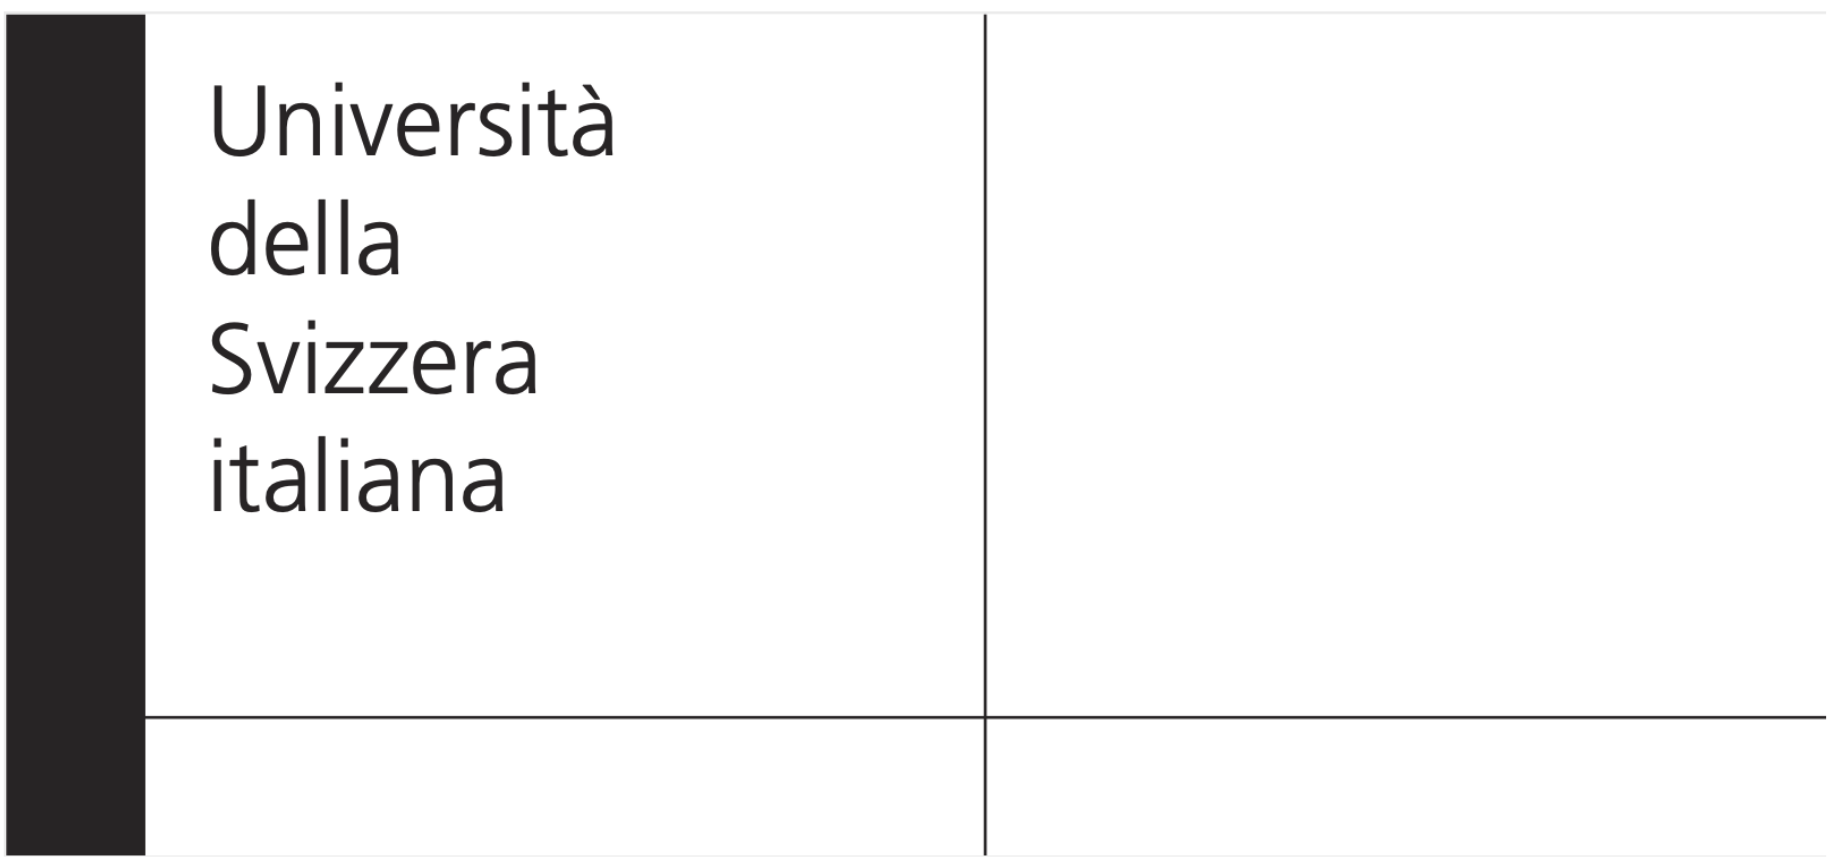
\includegraphics[width=0.4\textwidth]{images/usi_inf.png}
\end{flushleft}
  \noindent%
  {\large\ignorespaces{\textbf{#1}}\hspace{\fill}\ignorespaces{ \textbf{#2}}}\\ \\%
  {\large\ignorespaces #3 \hspace{\fill}\ignorespaces #4}\\
  \noindent%
  \bigskip
  \hrule\par\bigskip\noindent%
  \bigskip {\ignorespaces {\Large{\textbf{#5}}}
  \hspace{\fill}\ignorespaces \large \ifthenelse{\boolean{\isassignment}}{\duedate}{#6}}
  \hrule\par\bigskip\noindent%  \linebreak
 }

\makeatletter
\def\enumerateMod{\ifnum \@enumdepth >3 \@toodeep\else
      \advance\@enumdepth \@ne
      \edef\@enumctr{enum\romannumeral\the\@enumdepth}\list
      {\csname label\@enumctr\endcsname}{\usecounter
        {\@enumctr}%%%? the following differs from "enumerate"
	\topsep0pt%
	\partopsep0pt%
	\itemsep0pt%
	\def\makelabel##1{\hss\llap{##1}}}\fi}
\let\endenumerateMod =\endlist
\makeatother




\usepackage{textcomp}






\usepackage{subcaption}

\begin{document}


\setassignment

\serieheader{Particle Methods}{2022}{Student: Filippo Casari}{}{Report for Assignment 1}{}
\newline
\section*{Introduction}
My first approach for this assignment was using python. 
Although the logic behing the code seemed to work, by using $H>4$ as parameter, I got some 
troubles about the performances of the program. Consequently, I switched to Matlab to exploit multithreading and GPU power. \\
The program asks to users to decide whether to save the result image, to apply random search, and to choose the number H as well. 
\section*{Implementation}
I used 2 strategy for implementing the algorithm for moving the agents:
\begin{itemize}
    \item \textbf{Random search}: The unhappy agents move to a random position in the grid. The direction is chosen randomly. 
    \item \textbf{NN}: Nearest Neiighbour. The unhappy agents move to the nearest empty position in the grid. The direction goes from the left to the right, and from the top to the bottom.
\end{itemize}


Since it could happen for large number of H that the algorithm is going to converge very slowly or in the case of NN never converges, I implemented a so-called \textbf{early stopping} condition. 
It consists in checking if the number of unhappy agents is the same for 1000 consecutive iterations. If this happens, the algorithm stops. \\
Speaking about the best strategy, it turns out that the Random one is the best one. Indeed, sometimes the NN does not let the algorithm converge to 100 percent of happiness. \\
In contrast, the Random movement agent strategy for large H takes very long time to converge, and this leads to an early stopping criterion.\\
\section*{Results}
When the algorithm reaches 100 percent of happiness, the result image shows a really nice patterns which look like a sort of segregation between green and red points. 
\begin{figure}[H]
    
    \begin{subfigure}[b]{0.3\textwidth}
        \adjustbox{max height=\dimexpr\textheight-9\baselineskip}{
      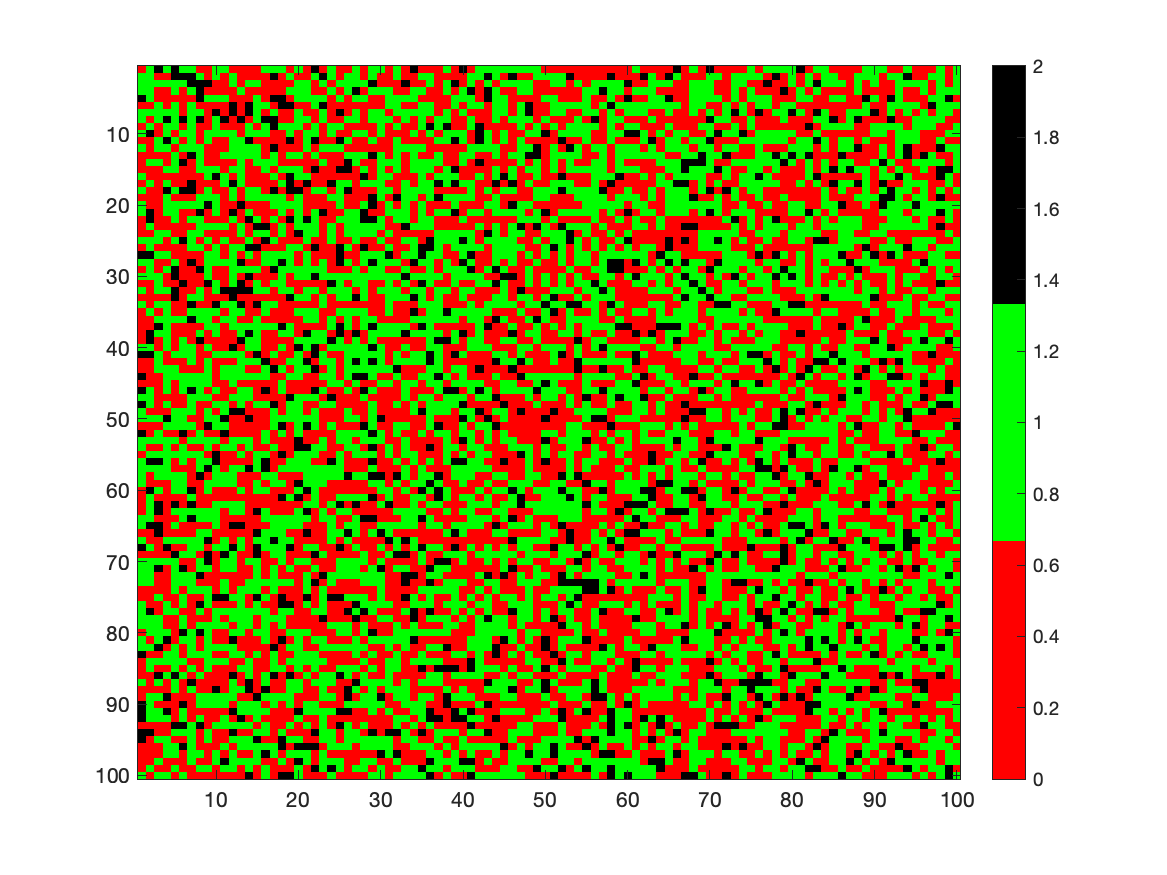
\includegraphics[width=\textwidth]{results/iterations_5_H_1_random_1.png}}
      \caption{Image 1}
      \label{fig:image1}
    \end{subfigure}
    \begin{subfigure}[b]{0.3\textwidth}
        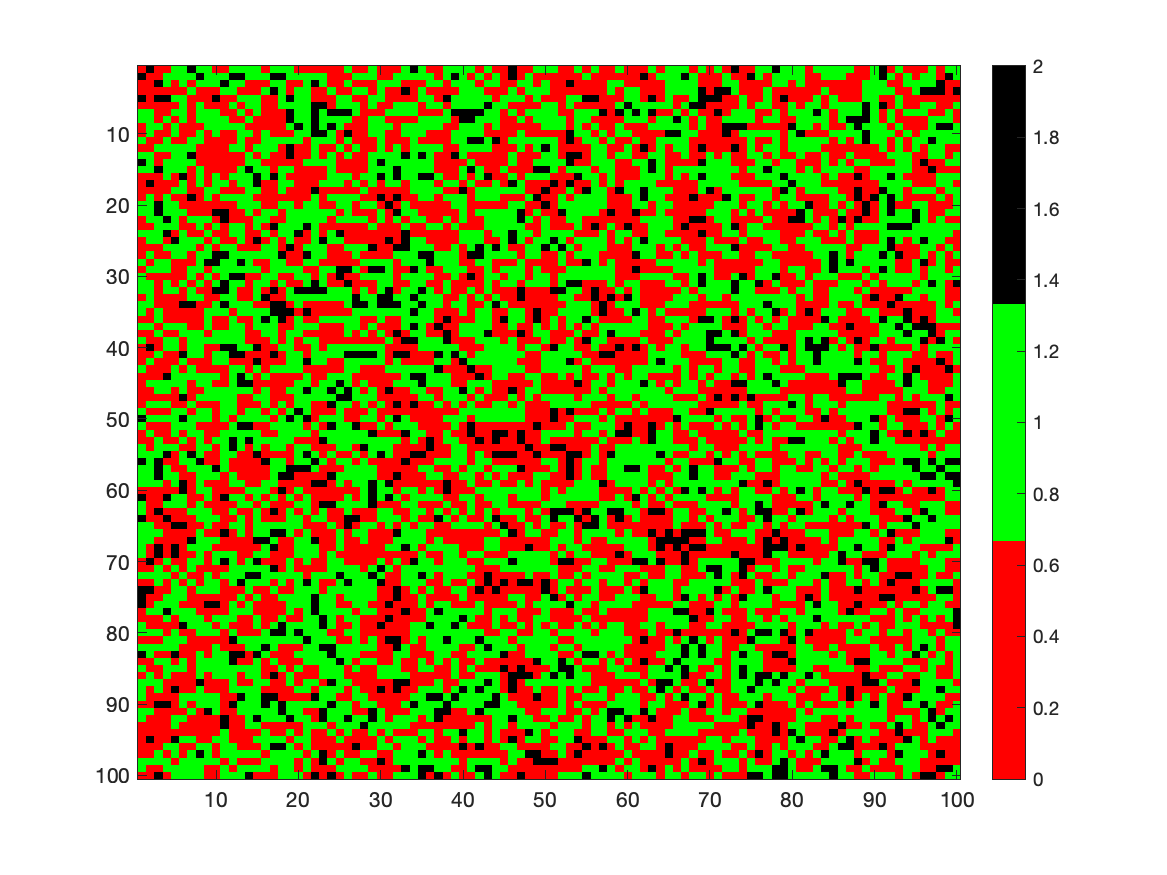
\includegraphics[width=\textwidth]{results/iterations_16_H_2_random_1.png}
        \caption{Image 2}
        \label{fig:image2}
      \end{subfigure}
      \begin{subfigure}[b]{0.3\textwidth}
        \adjustbox{max height=\dimexpr\textheight-9\baselineskip}{
        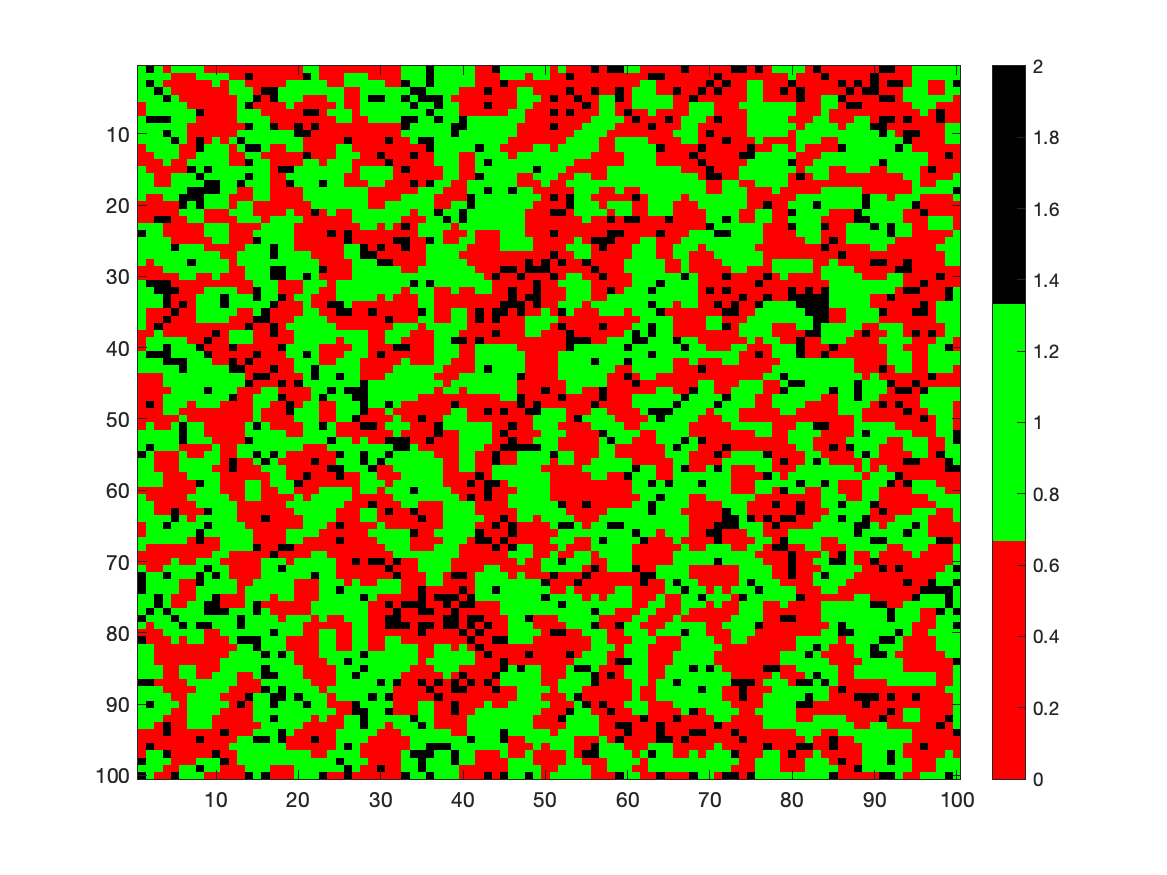
\includegraphics[width=\textwidth]{results/iterations_64_H_3_random_1.png}}
        \caption{Image 3}
        \label{fig:image3}
      \end{subfigure}
      \begin{subfigure}[b]{0.3\textwidth}
        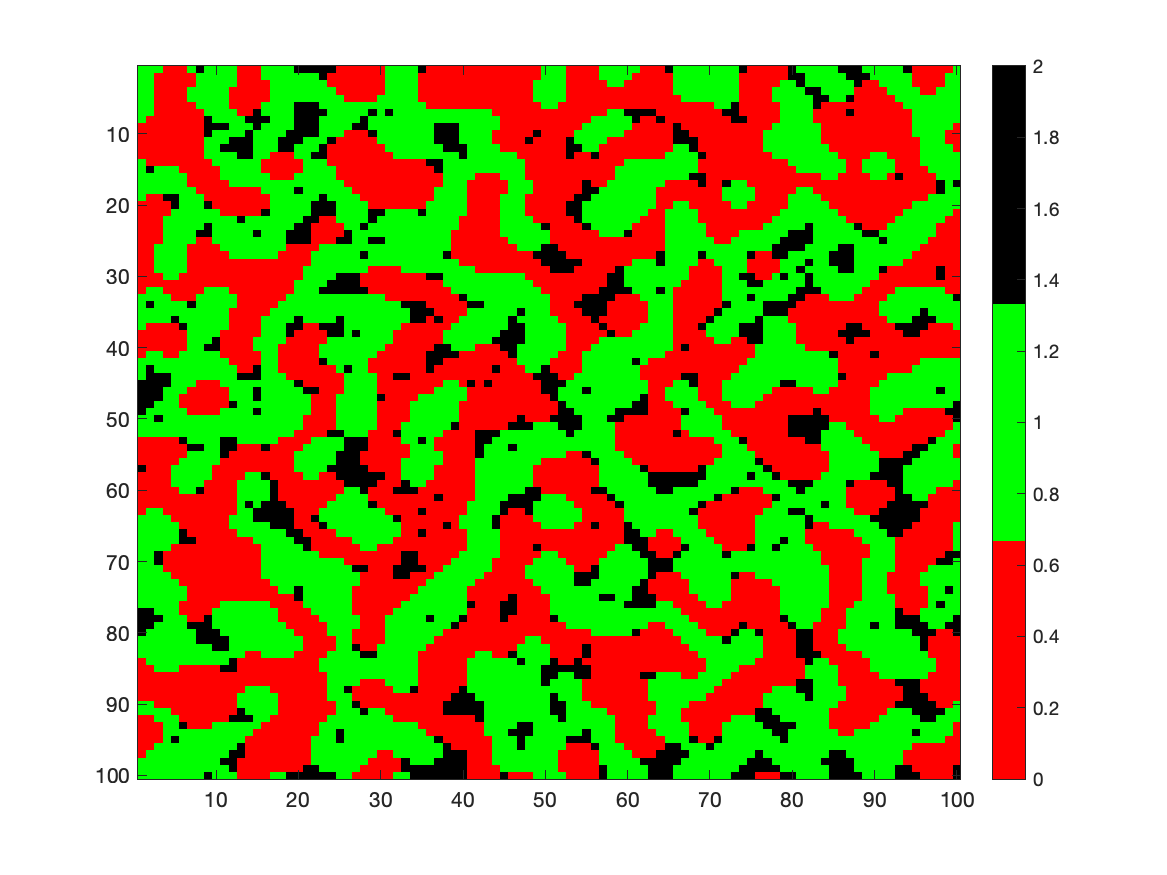
\includegraphics[width=\textwidth]{results/iterations_196_H_4_random_1.png}
        \caption{Image 4}
        \label{fig:image4}
      \end{subfigure}
      \begin{subfigure}[b]{0.3\textwidth}
        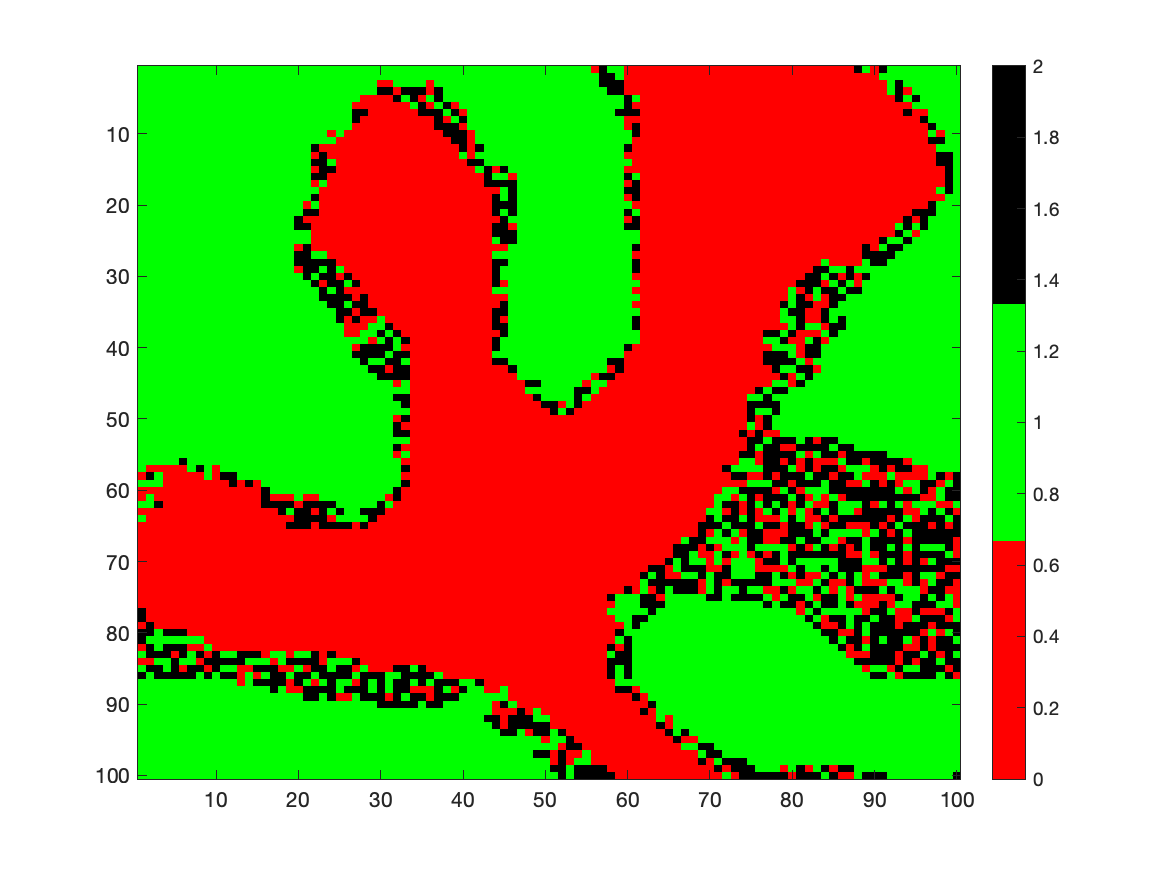
\includegraphics[width=\textwidth]{results/iterations_1888_H_5_random_1.png}
        \caption{Image 5}
        \label{fig:image5}
      \end{subfigure}
      \begin{subfigure}[b]{0.3\textwidth}
        \adjustbox{max height=\dimexpr\textheight-9\baselineskip}{
        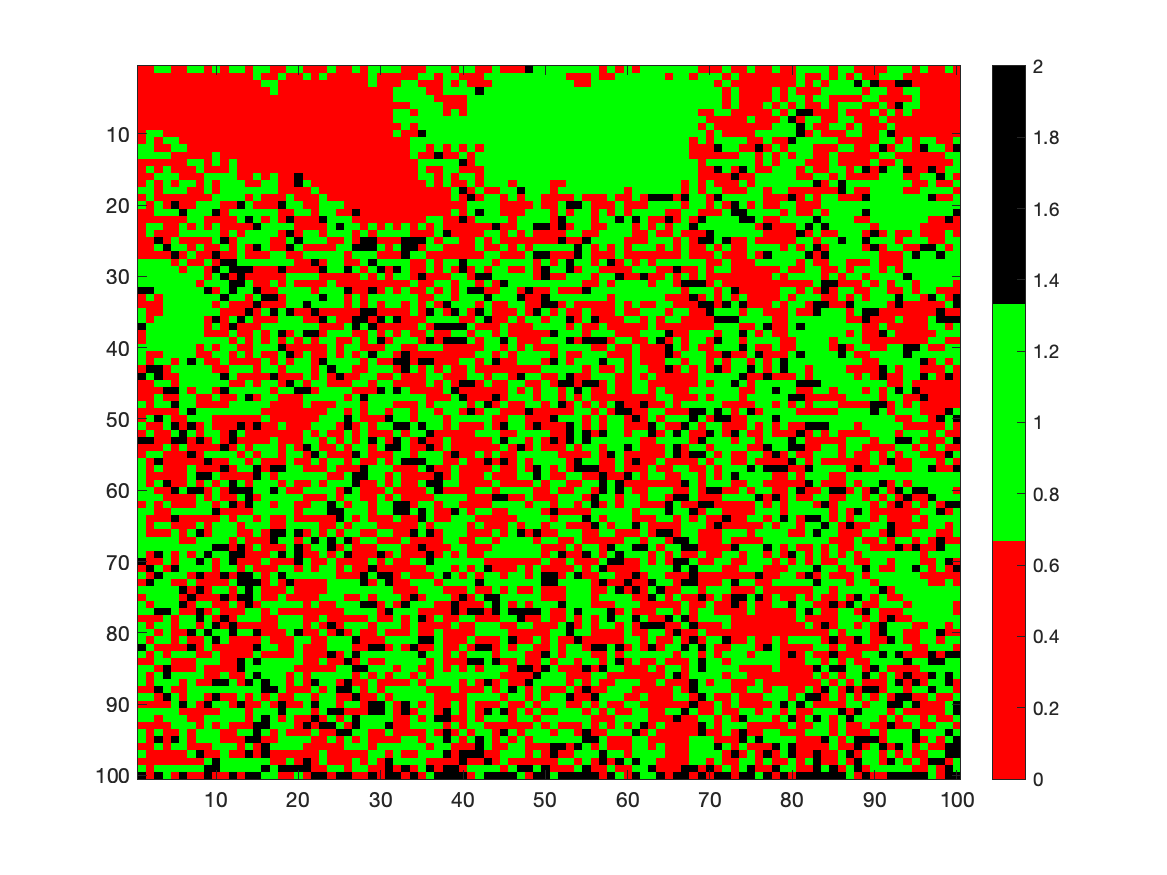
\includegraphics[width=\textwidth]{results/iterations_2261_H_6_random_1.png}}
        \caption{Image 6}
        \label{fig:image6}
      \end{subfigure}
      
      \begin{subfigure}[b]{0.3\textwidth}
        \adjustbox{max height=\dimexpr\textheight-9\baselineskip}{
        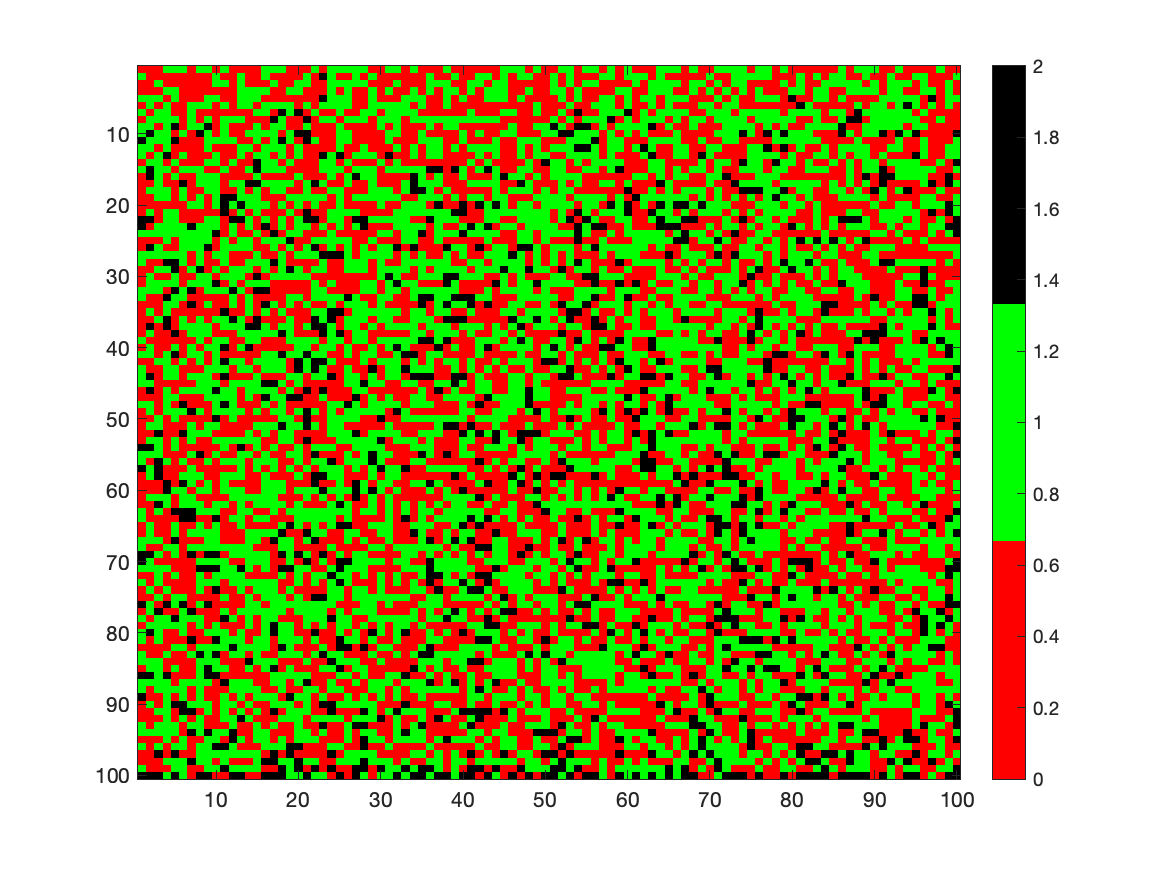
\includegraphics[width=\textwidth]{results/iterations_1056_H_7_random_1.png}}
        \caption{Image 7}
        \label{fig:image7}
      \end{subfigure}
      \begin{subfigure}[b]{0.3\textwidth}
        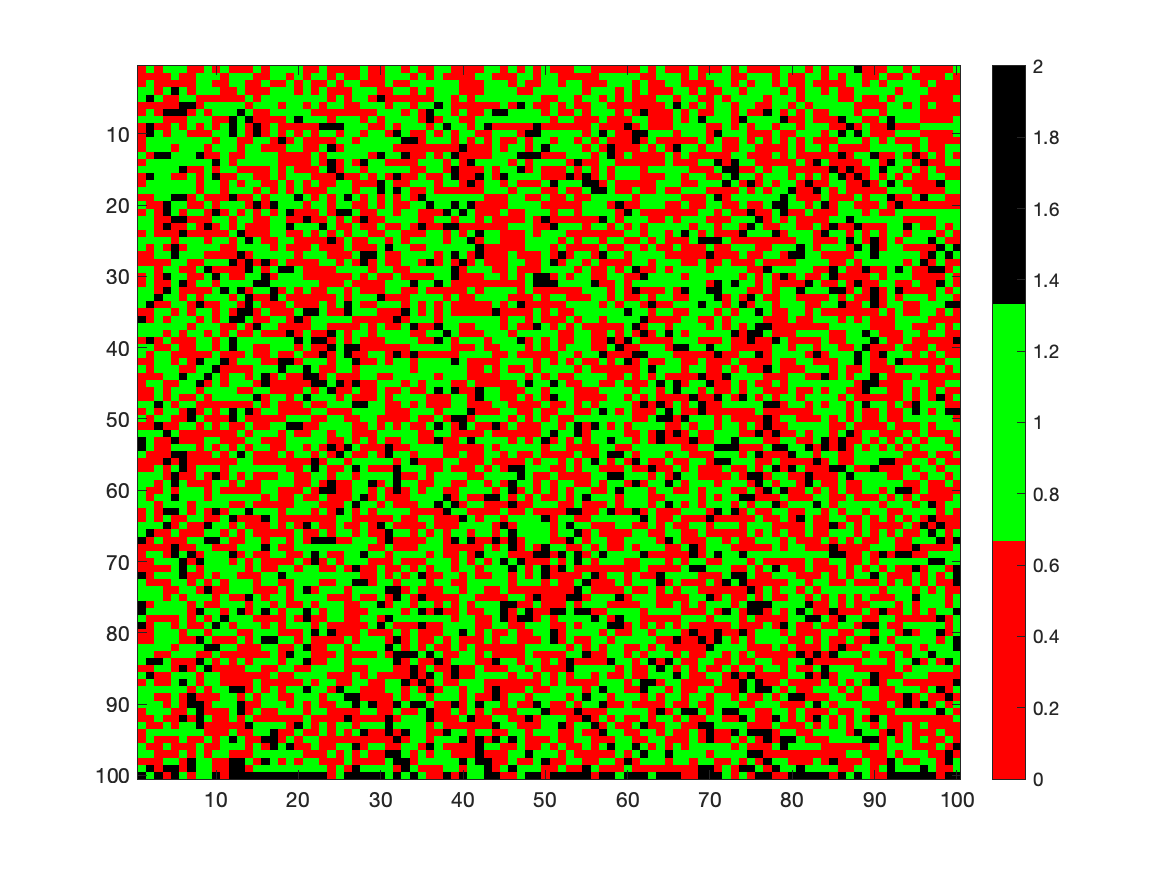
\includegraphics[width=\textwidth]{results/iterations_1002_H_8_random_1.png}
        \caption{Image 8}
        \label{fig:image8}
      \end{subfigure}
      \begin{subfigure}[b]{0.3\textwidth}
        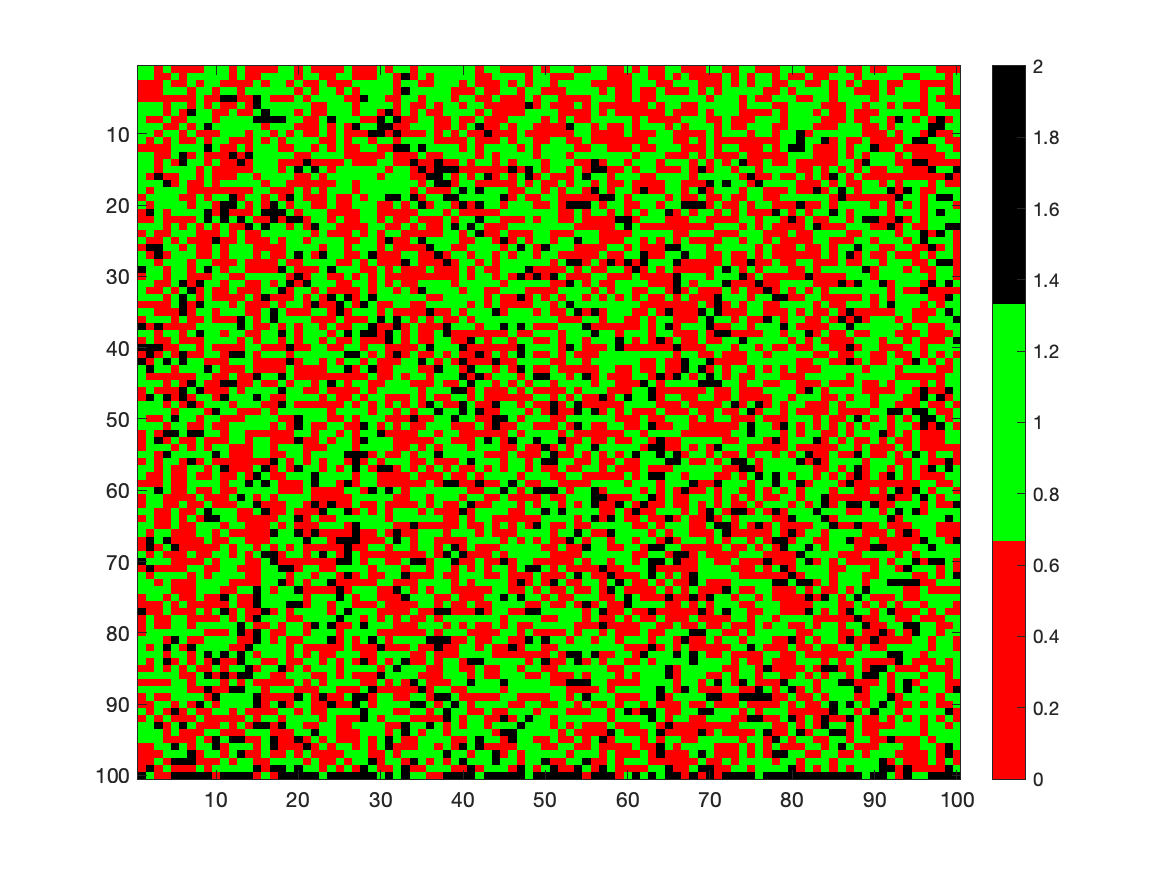
\includegraphics[width=\textwidth]{results/iterations_1002_H_9_random_1.png}
        \caption{Image 9}
        \label{fig:image9}
      \end{subfigure}
      
\end{figure}
I reported above the grids at the end of the algorithm for different values of H and Random=True. 
I also saved the grids for Random=False (NN) in "results" directory. \\
It turns out that with $H>5$ (from image 6) the segregation is not so clear or there isn't at all. \\
Below I reported also the level (percentage) of happiness for each case. If the level si not 100 percent is because maybe the algorithm converges to a local "minimum" or because of the early stopping criterion was met. This could happen if the happiness did not improve within a time window of 1000 iterations. 
\begin{figure}[H]
    
    \begin{subfigure}[b]{0.4\textwidth}
        
      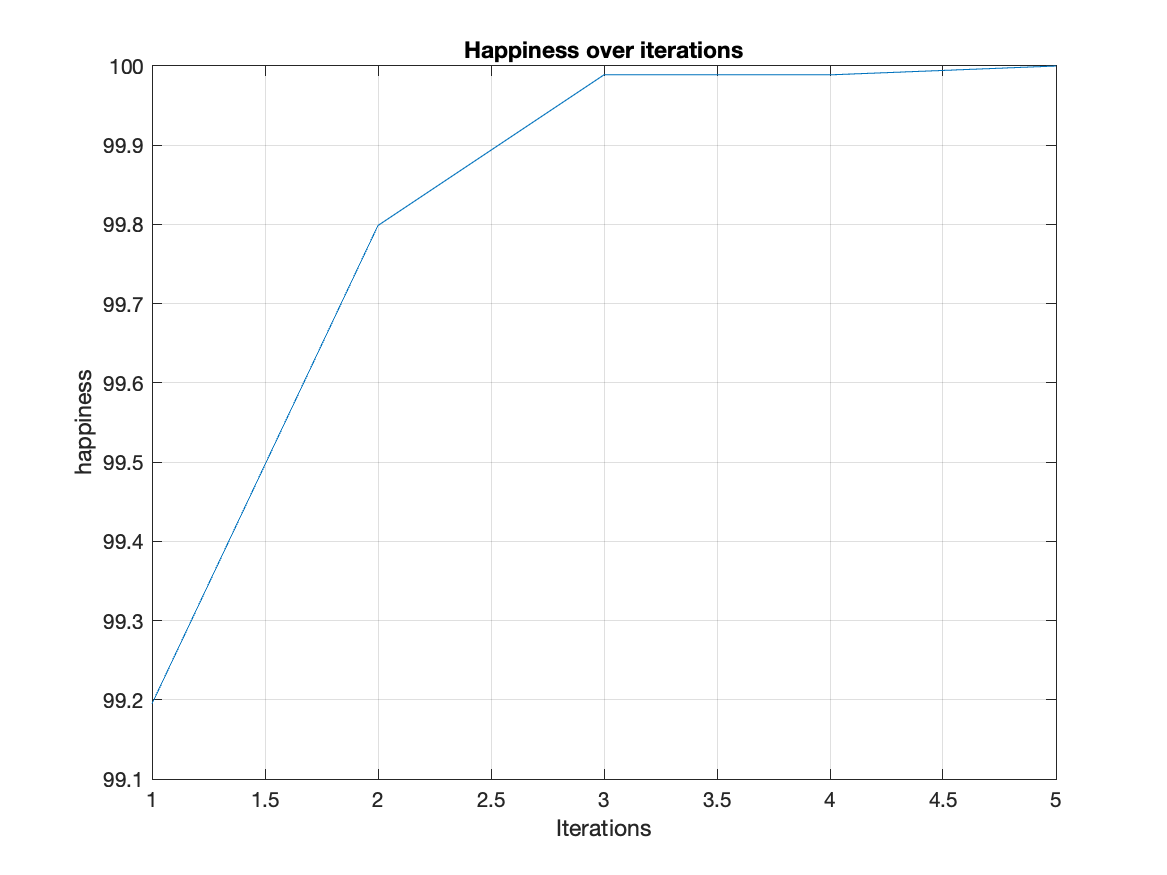
\includegraphics[width=\textwidth]{Convergence/ConvergenceH1Random_1.png}
      \caption{Image 1}
      \label{fig:image1}
    \end{subfigure}
    \begin{subfigure}[b]{0.4\textwidth}
        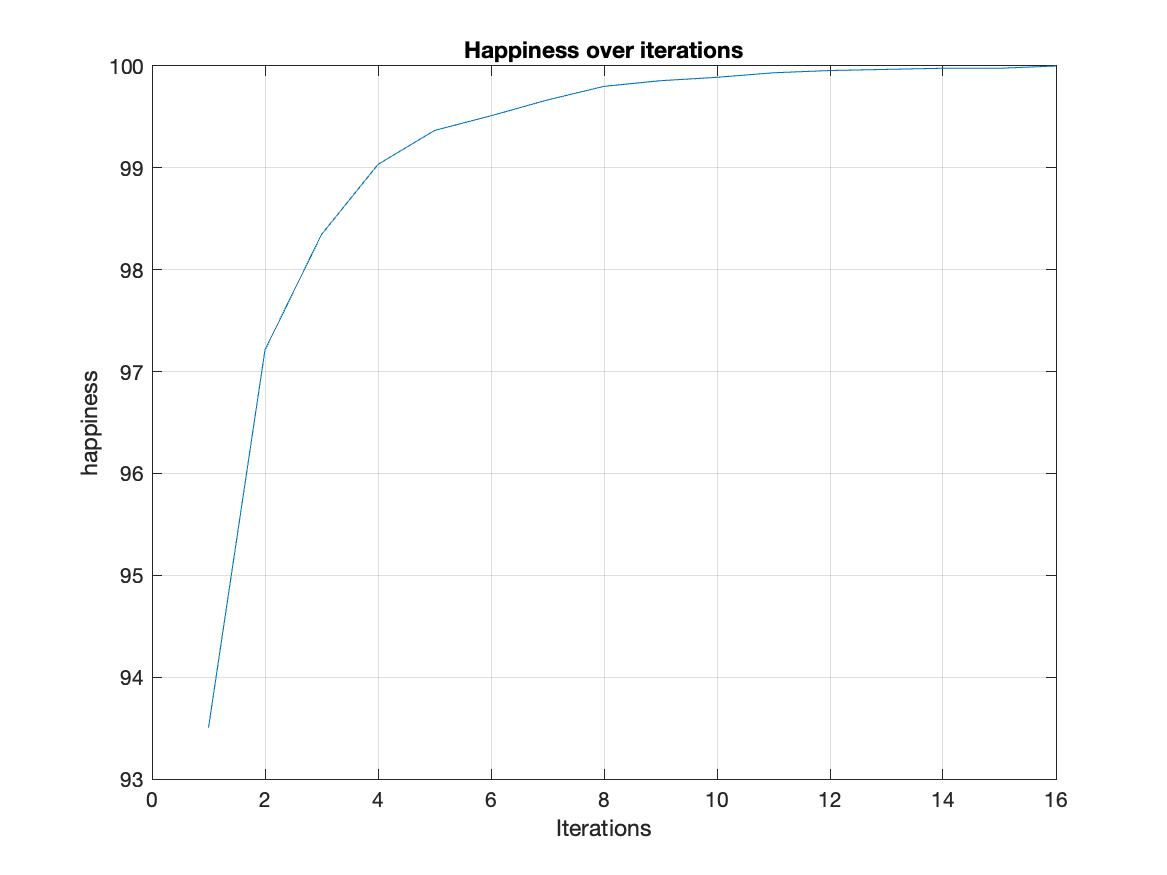
\includegraphics[width=\textwidth]{Convergence/ConvergenceH2Random_1.png}
        \caption{Image 2}
        \label{fig:image2}
      \end{subfigure}
      \begin{subfigure}[b]{0.4\textwidth}
        
        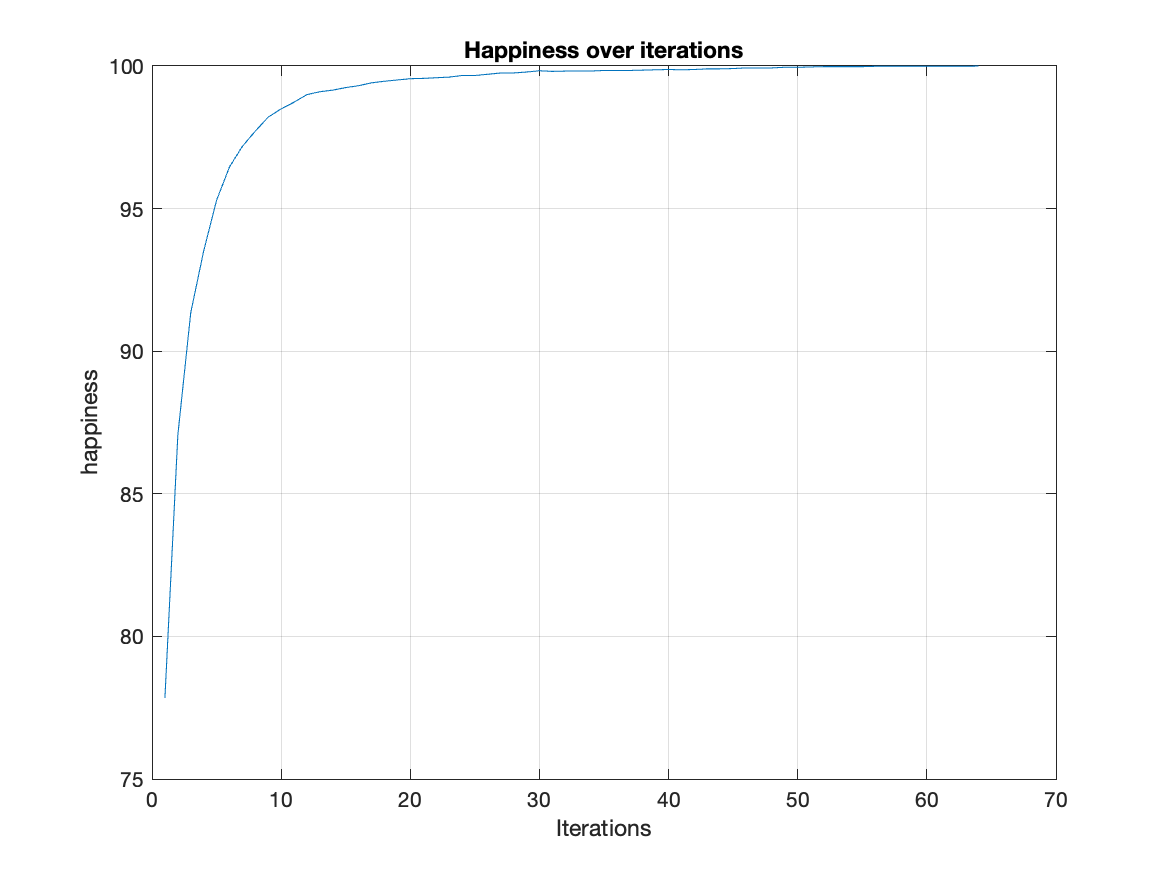
\includegraphics[width=\textwidth]{Convergence/ConvergenceH3Random_1.png}
        \caption{Image 3}
        \label{fig:image3}
      \end{subfigure}
      \begin{subfigure}[b]{0.4\textwidth}
        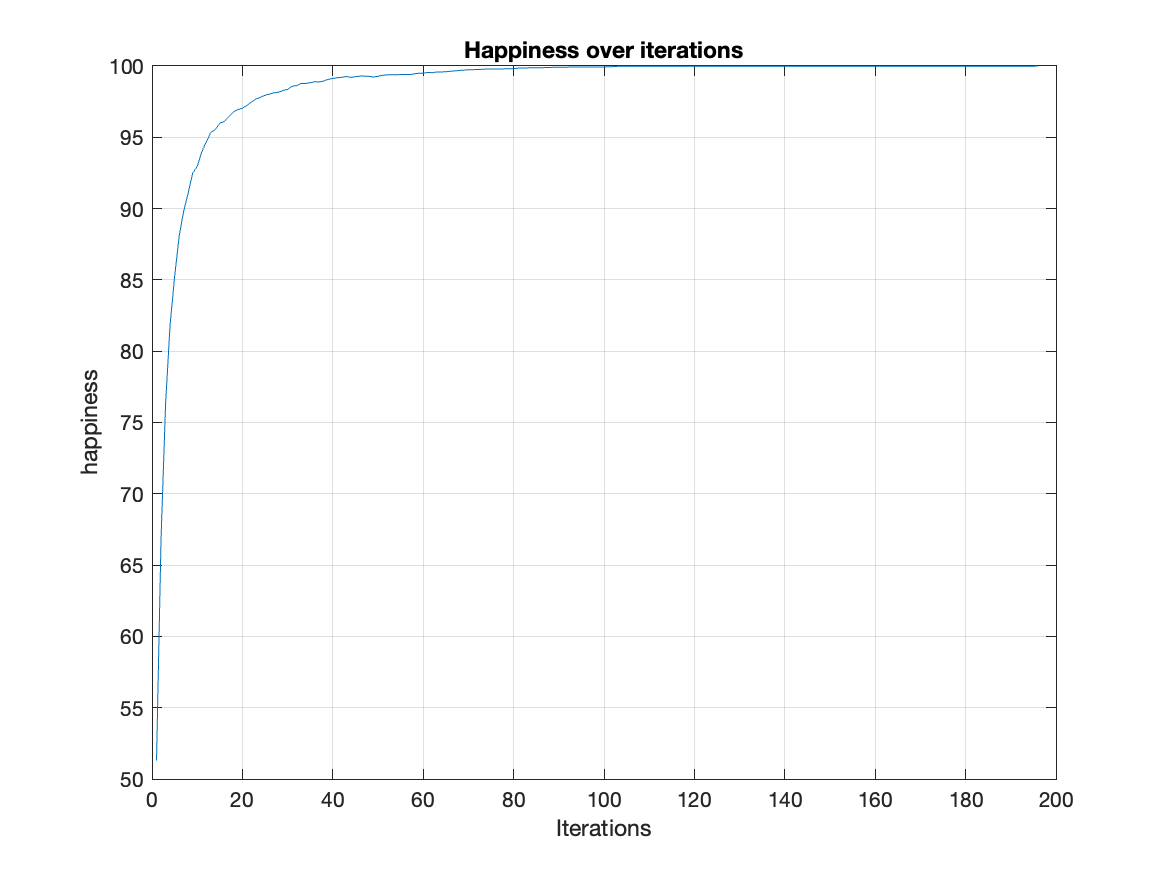
\includegraphics[width=\textwidth]{Convergence/ConvergenceH4Random_1.png}
        \caption{Image 4}
        \label{fig:image4}
      \end{subfigure}
      \begin{subfigure}[b]{0.4\textwidth}
        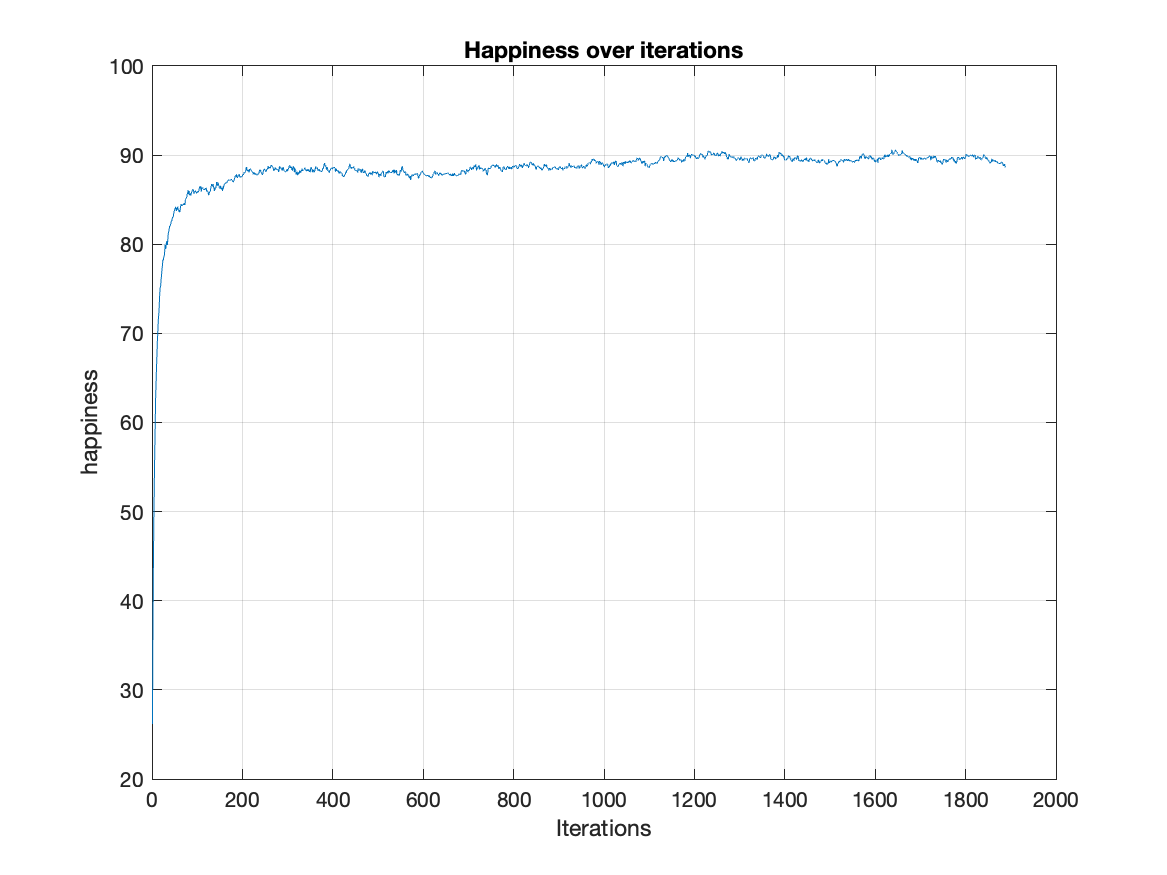
\includegraphics[width=\textwidth]{Convergence/ConvergenceH5Random_1.png}
        \caption{Image 5}
        \label{fig:image5}
      \end{subfigure}
      \begin{subfigure}[b]{0.4\textwidth}
        
        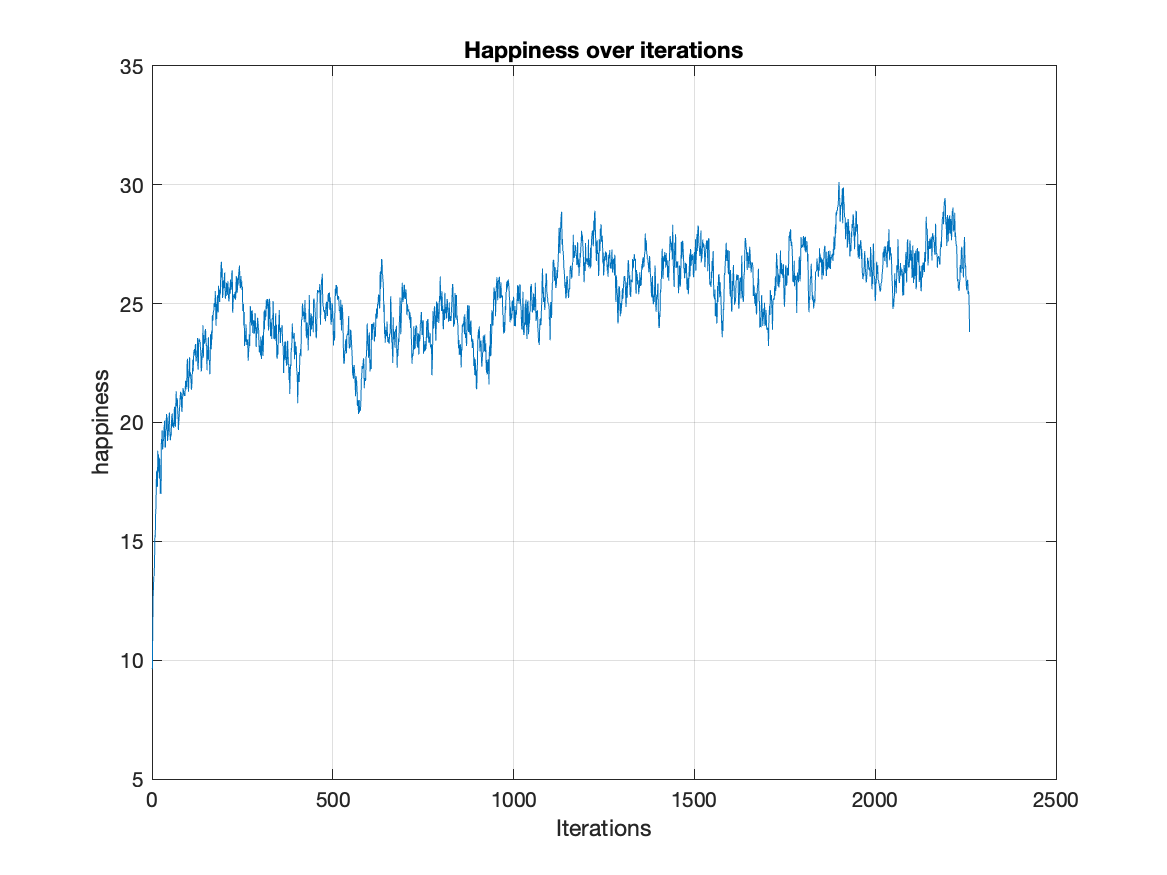
\includegraphics[width=\textwidth]{Convergence/ConvergenceH6Random_1.png}
        \caption{Image 6}
        \label{fig:image6}
      \end{subfigure}
      
      \begin{subfigure}[b]{0.4\textwidth}
        
        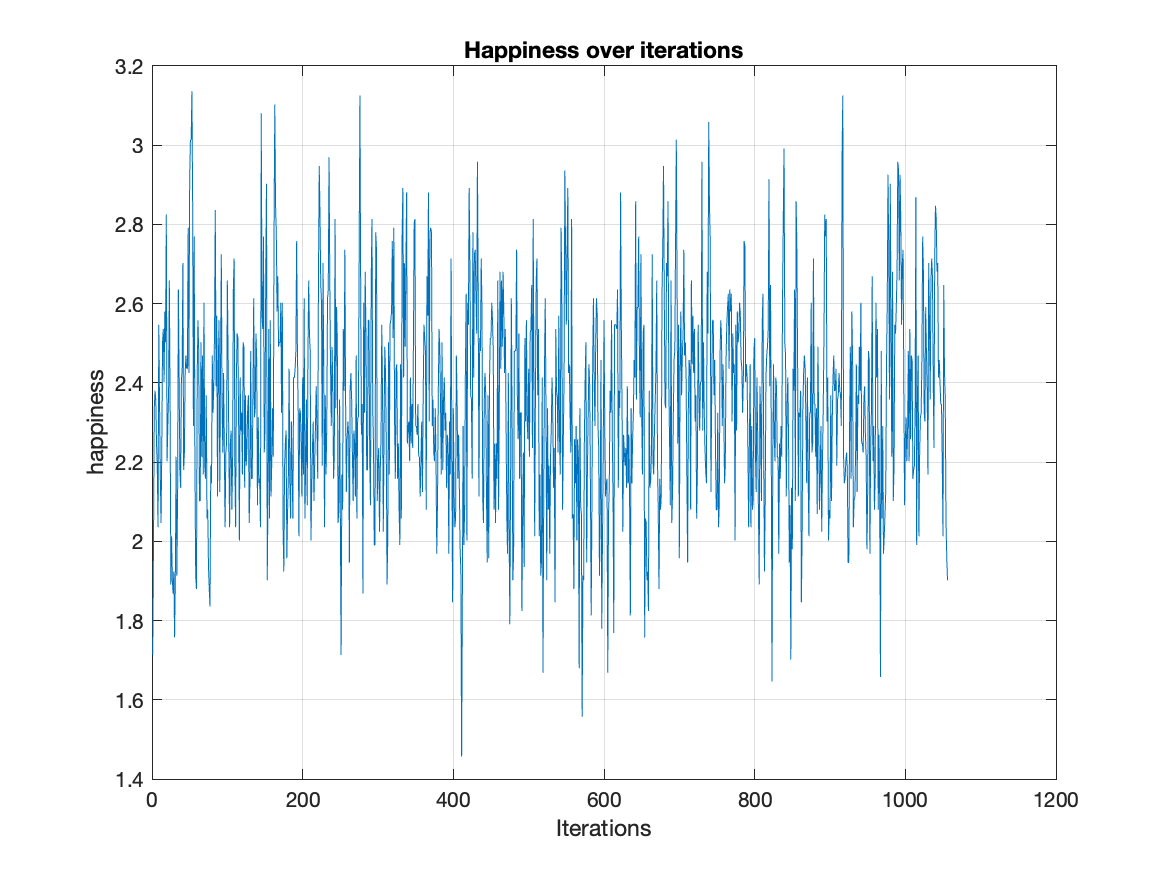
\includegraphics[width=\textwidth]{Convergence/ConvergenceH7Random_1.png}
        \caption{Image 7}
        \label{fig:image7}
      \end{subfigure}
      \begin{subfigure}[b]{0.4\textwidth}
        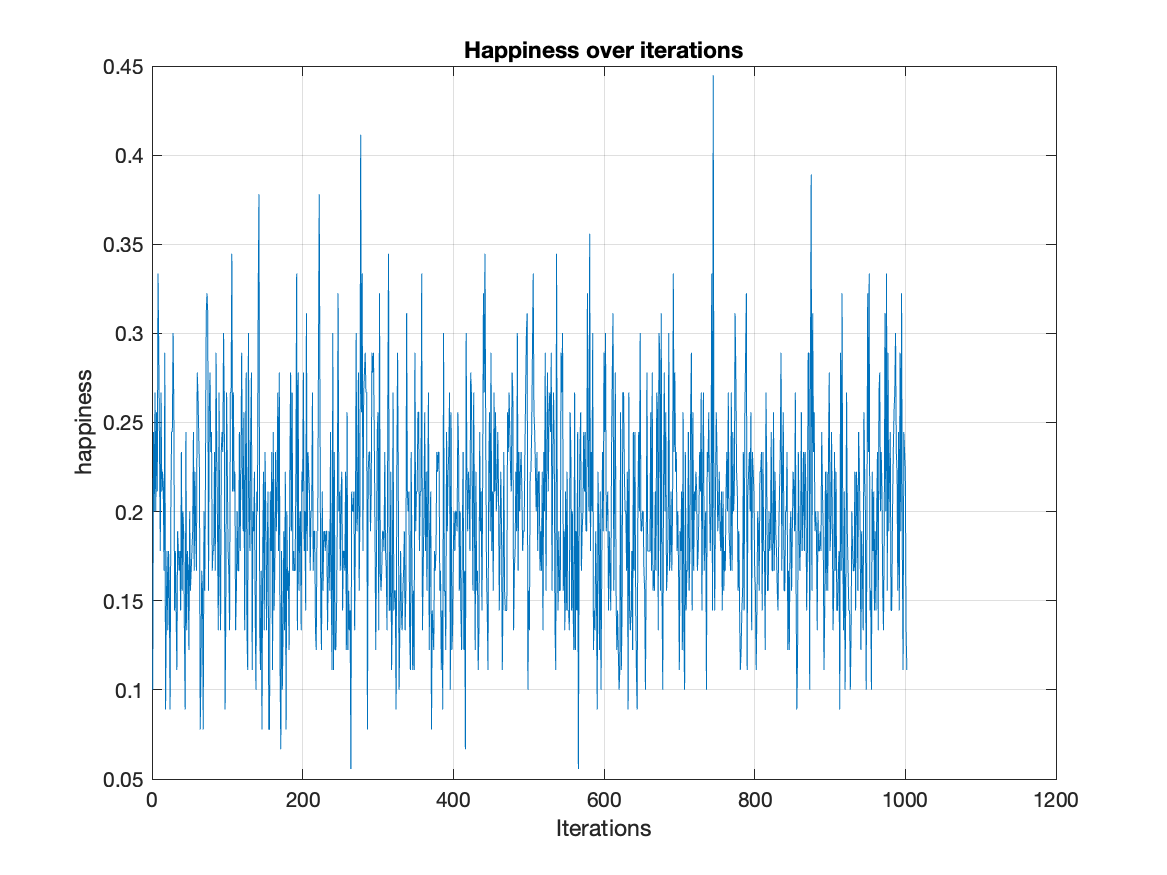
\includegraphics[width=\textwidth]{Convergence/ConvergenceH8Random_1.png}
        \caption{Image 8}
        \label{fig:image8}
      \end{subfigure}
      
      
\end{figure}
As one can see the heppiness with $H<6$ it converges whereas with H higher the level is going up and down without reaching a good level of happiness. \\
\end{document}
